%!TEX TS-program = xelatex
\documentclass[aspectratio=169]{beamer}
\usepackage{tikz}
\usepackage{calc}
% \usepackage{polyglossia}
% \setmainlanguage{vietnamese}
% Thay thế bằng fontspec để tránh lỗi polyglossia
\usepackage{fontspec}
\setmainfont{Times New Roman}
\usepackage{amsthm,amsmath,amssymb}
\newtheorem{thm}{Định lý}
\newtheorem{defn}{Định nghĩa}
\usepackage{subcaption}
\setbeamertemplate{theorems}[numbered]

%% TYPESET
\makeatletter
\newcommand{\leqnomode}{\tagsleft@true}
\newcommand{\reqnomode}{\tagsleft@false}
\makeatother
\let\Mathcal\mathcal
% \usepackage{dutchcal}  % Commented out to avoid font errors
\newcommand{\norm}[1]{\left\lVert#1\right\rVert}
\newcommand{\abs}[1]{\left\lvert#1\right\rvert}
\newcommand{\gr}{\operatorname{gr}}
\newcommand{\rank}{\operatorname{rank}}
\newcommand{\toto}{\rightrightarrows}%
\newcommand{\F}{\Mathcal{F}}%
\newcommand{\K}{\mathbb{K}}%
\newcommand{\R}{\mathbb{R}}%
\def\C{\mathbb{C}}%
\newcommand{\dom}{\operatorname{dom}}%
% \newcommand{\ker}{\operatorname{ker}}% already defined
\newcommand{\im}{\operatorname{im}}%
\newcommand{\g}{\mathcal{g}}%
\global\long\def\MP{\text{mp}}%

\newcommand{\Image}[1]{%
	\sbox0{\includegraphics[height=0.65\paperheight]{#1}}%
	\ifdim\wd0 < \textwidth
	\includegraphics[height=0.65\paperheight]{#1}%
	\else
	\includegraphics[width=\textwidth]{#1}%
	\fi%
}


\newif\iffirsttoc
\firsttoctrue
\AtBeginSection[]
{
    \begin{frame}
        \frametitle{Mục lục}  
        \iffirsttoc
            \tableofcontents
            \global\firsttocfalse
        \else
            \tableofcontents[currentsection,
            % hideothersubsections,
            subsectionstyle=show/shaded/hide,
            subsubsectionstyle=show/show/show/hide
            ]
        \fi
    \end{frame} 
}

\setbeamertemplate{caption}[numbered]

\usetheme{hust}
% \titlegraphic{\includegraphics[height=\logoheight]{figures/sami-v2.pdf}}
\title{Đồ án II}
\subtitle{\textbf{VRAE: Cải tiến bộ mã hóa tự động \\ khử nhiễu và khử mờ cho biển số xe}}
% \subtitle{\textbf{khử nhiễu và khử mờ cho biển số xe}}

\author{Sinh viên thực hiện: Nguyễn Tất Cường - 202227090\\Giảng viên hướng dẫn: TS. Trần Ngọc Thăng\\Khoa Toán Tin -- Đại học Bách Khoa Hà Nội}
\date{Tháng 01, 2026}

\begin{document}
\begin{frame}[noframenumbering,Title]
	\maketitle
\end{frame}

\section{Đặt vấn đề}

\begin{frame}{Đặt vấn đề}
    \begin{itemize}
        \item \textbf{Thực trạng:} Ảnh giám sát giao thông thường bị suy giảm chất lượng do:
        \begin{itemize}
            \item Điều kiện ánh sáng kém, thời tiết xấu gây nhiễu
            \item Chuyển động nhanh gây mờ 
            \item Giới hạn phần cứng thiết bị ghi/xử lý hình ảnh
        \end{itemize}
        \item \textbf{Hậu quả:}
        \begin{itemize}
            \item Giảm độ chính xác của hệ thống nhận diện biển số (ANPR/OCR)
            \item Sai lệch trong xử lý vi phạm và quản lý giao thông
            \item Ảnh hưởng đến điều tra an ninh
        \end{itemize}
        \item \textbf{Thách thức:}
        \begin{itemize}
            \item Cần bảo toàn chi tiết ảnh để không ảnh hưởng các thao tác nhận diện biển số
            \item Yêu cầu xử lý thời gian thực trên thiết bị nhúng
        \end{itemize}
        \item \textbf{Giải pháp:}
        \begin{itemize}
            \item Kiến trúc cải tiến của mã hóa tự động có bổ sung thiết kế phụ trợ để cải tiến khả năng khôi phục ảnh và tối ưu tham số mô hình 
        \end{itemize}
    \end{itemize}
\end{frame}

\begin{frame}{Bài báo tại hội nghị SOICT 2025}
    \begin{columns}
        \begin{column}{0.5\textwidth}
            \begin{figure}
                \centering
                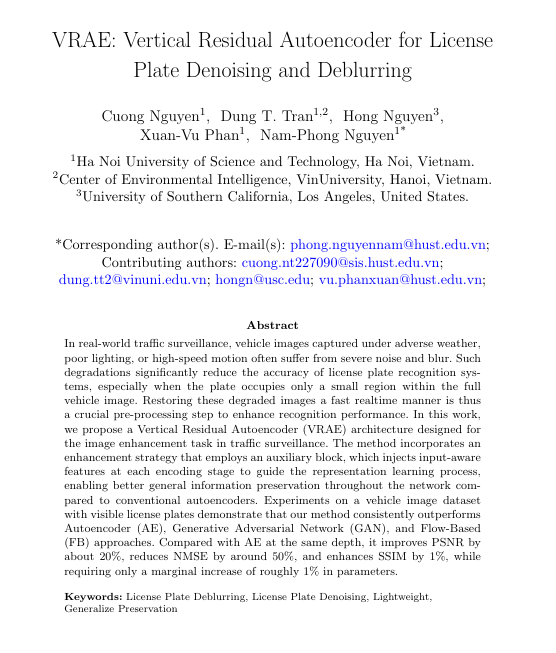
\includegraphics[width=\linewidth]{images/first_page_paper.png}
                % \caption{Thay đổi Entropy }
            \end{figure}
        \end{column}
        \begin{column}{0.4\textwidth}
            \textbf{Hội nghị SOICT 2025}
            \begin{itemize}
                \item Hội nghị quốc tế lần thứ 14 về công nghệ thông tin và truyền thông
                \item Năm 2025, SOICT thu hút hơn 327 bài gửi từ 30 quốc gia.
                \item Lĩnh vực: Khoa học máy tính, trí tuệ nhân tạo, khoa học dữ liệu, thông tin và truyền thông, v.v.
            \end{itemize}
        \end{column}
    \end{columns}
\end{frame}

% \subsection{Mục tiêu nghiên cứu}
% \begin{frame}{Mục tiêu nghiên cứu}
%     \small
%     \begin{enumerate}
%         \item Đề xuất phương pháp khử nhiễu và khử mờ hiệu quả cho ảnh phương tiện, tập trung vào việc bảo toàn chi tiết vùng biển số
%         \item Tối ưu hóa mô hình về số tham số và chi phí tính toán để phù hợp triển khai trên thiết bị thực tế
%         \item Đánh giá hiệu quả bằng các chỉ số ảnh kỹ thuật (PSNR, SSIM) và tỷ lệ nhận diện biển số sau xử lý
%     \end{enumerate}
    
%     \vspace{0.1cm}
%     \textbf{Đo lường hiệu quả:}
%     \begin{itemize}
%         \item PSNR (Peak Signal-to-Noise Ratio)
%         \item SSIM (Structural Similarity Index)
%         \item NMSE (Normalized Mean Squared Error)
%         \item Thời gian xử lý và kích thước mô hình
%     \end{itemize}
% \end{frame}


\section{Phát biểu bài toán}

\begin{frame}{Phát biểu bài toán}
    Cho một ảnh quan sát $Y$ chứa phương tiện và vùng biển số bị suy giảm do nhiễu và/hoặc mờ, mục tiêu là tìm một ảnh ước lượng $\hat{X}$ gần với ảnh nguyên gốc $X$.
    
    \vspace{0.5cm}
    Mô hình tổng quát:
    \begin{equation}
        Y = K * X + N
    \end{equation}
    trong đó:
    \begin{itemize}
        \item $K$: hạt nhân làm mờ (blur kernel)
        \item $*$: phép nhân chập
        \item $N$: thành phần nhiễu (Gaussian, Poisson, sensor noise)
    \end{itemize}
    
    \vspace{0.3cm}
    Nhiệm vụ: Ước lượng $\hat{X}$ và (nếu cần) $K$ từ $Y$.
\end{frame}


\section{Khoảng trống nghiên cứu}

\begin{frame}{Khoảng trống nghiên cứu}
    \begin{table}[]
        \centering
        \tiny % Reduce font size to fit better
        \setlength{\tabcolsep}{3pt} % Reduce column padding
        \renewcommand{\arraystretch}{1.2} % Adjust row height
        \resizebox{\textwidth}{!}{%
        \begin{tabular}{|l|l|l|}
        \hline
        \textbf{Phương pháp} & \textbf{Ưu điểm} & \textbf{Hạn chế} \\ \hline
        \textbf{AE} & 
        \begin{minipage}{0.3\textwidth}
        \begin{itemize}
            \item Gọn nhẹ
            \item Phù hợp hệ thống giám sát
        \end{itemize}
        \end{minipage} & 
        \begin{minipage}{0.3\textwidth}
        \begin{itemize}
            \item Mất mát thông tin tần số cao
            \item Thất bại với cấu trúc trung/cao cấp
        \end{itemize}
        \end{minipage} \\ \hline
        \textbf{GAN} & 
        \begin{minipage}{0.3\textwidth}
        \begin{itemize}
            \item Ảnh sắc nét, chân thực
            \item Cải thiện perceptual quality
        \end{itemize}
        \end{minipage} & 
        \begin{minipage}{0.3\textwidth}
        \begin{itemize}
            \item Biến dạng độ trung thực pixel
            \item Dễ sinh chi tiết giả (hallucination)
            \item Khó huấn luyện
        \end{itemize}
        \end{minipage} \\ \hline
        \textbf{FB} & 
        \begin{minipage}{0.3\textwidth}
        \begin{itemize}
            \item Bảo toàn độ chính xác pixel
            \item Ánh xạ khả nghịch
        \end{itemize}
        \end{minipage} & 
        \begin{minipage}{0.3\textwidth}
        \begin{itemize}
            \item Độ phức tạp tính toán cao
            \item Tốn bộ nhớ lớn
        \end{itemize}
        \end{minipage} \\ \hline
        \end{tabular}%
        }
    \end{table}
    \vspace{0.1cm}
    \begin{block}{Khoảng trống nghiên cứu}
        Thiết kế mô hình \textbf{nhẹ, thời gian thực} nhưng vẫn \textbf{bảo toàn chi tiết chính xác} cho tăng cường ảnh giao thông.
    \end{block}
\end{frame}


\section{Phương pháp đề xuất}
\begin{frame}{Tổng quan phương pháp VRAE}
    \textbf{Vertical Residual Autoencoder (VRAE)} - Kiến trúc nhẹ chuyên dụng cho khử nhiễu và khử mờ biển số xe.
    
    \begin{columns}
        \begin{column}{0.5\textwidth}
            \begin{itemize}
                % \item \textbf{Mục tiêu:} Duy trì fidelity (PSNR/SSIM), bảo toàn chi tiết vi mô, đạt hiệu năng tính toán phù hợp thời gian thực
                \item \textbf{Backbone:} ResNet-50 (cân bằng năng lực và chi phí)
                \item \textbf{Đặc điểm:} Kết nối dọc + khối bổ trợ
            \end{itemize}
        \end{column}
        \begin{column}{0.65\textwidth}
            \begin{figure}
                \centering
                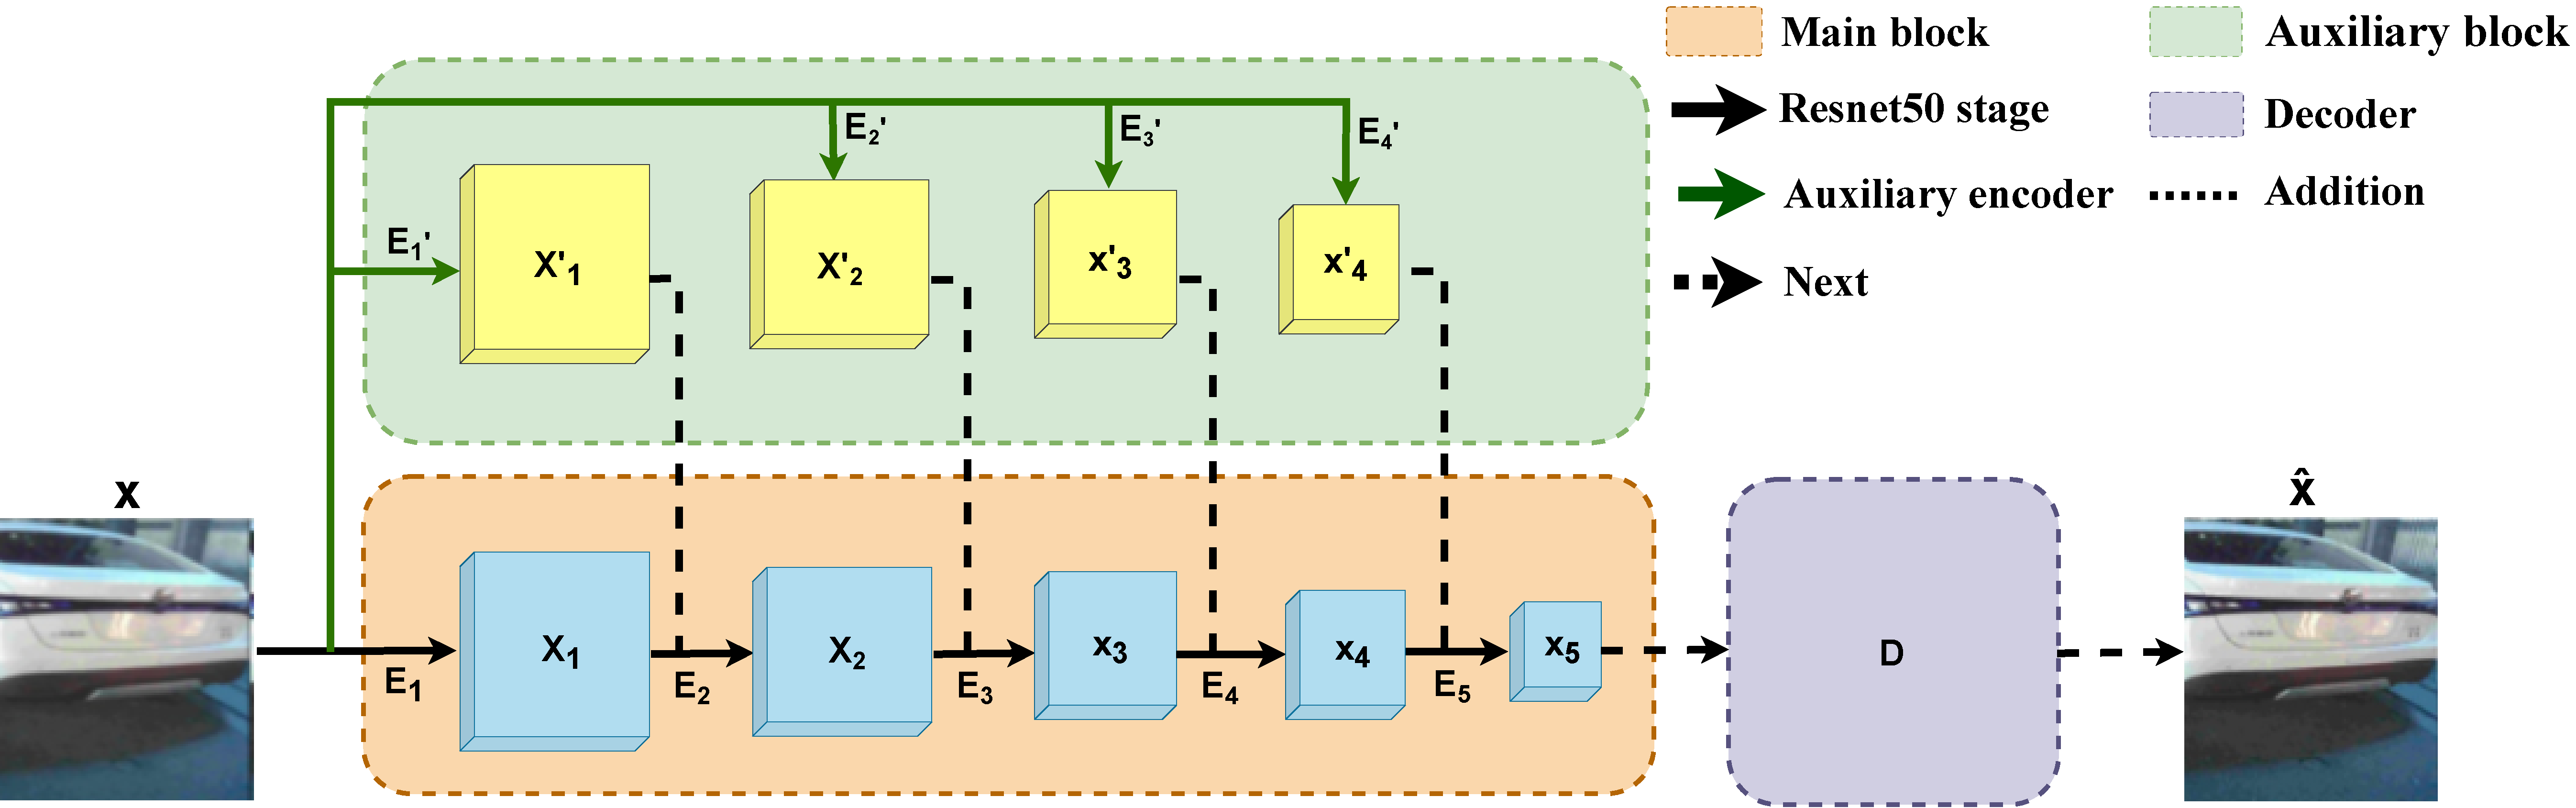
\includegraphics[width=0.9\linewidth]{images/VRAE.pdf}
                \caption{Kiến trúc VRAE}
            \end{figure}
        \end{column}
    \end{columns}
\end{frame}

\begin{frame}{Khối chính (Main Block)}
    \begin{columns}
        \begin{column}{0.4\textwidth}
            \textbf{Cấu trúc:}
            \begin{itemize}
                \item Dựa trên ResNet-50 (Stage 1-5)
                \item Cấu trúc Bottleneck:
                \begin{itemize}
                    \item $1 \times 1$: Giảm chiều
                    \item $3 \times 3$: Xử lý không gian
                    \item $1 \times 1$: Khôi phục kênh
                \end{itemize}
                \item Skip-connection: Cải thiện gradient flow
            \end{itemize}
        \end{column}
        \begin{column}{0.5\textwidth}
            \textbf{Kết nối dọc:}
            \begin{equation}
                \mathbf{x}_i = E_i(\mathbf{x}_{i-1} + \mathbf{x}'_{i-1})
            \end{equation}
            \begin{itemize}
                \item $\mathbf{x}_{i-1}$: Đầu ra khối chính
                \item $\mathbf{x}'_{i-1}$: Đầu ra khối bổ trợ
                \item Hội tụ đặc trưng đa cấp
            \end{itemize}
        \end{column}
    \end{columns}
\end{frame}

% \subsection{Khối bổ trợ}
\begin{frame}{Khối bổ trợ (Auxiliary Block)}
    \textbf{Mục đích:} Tăng cường khả năng giữ lại thông tin cục bộ và ngữ cảnh
    
    \vspace{0.3cm}
    \begin{columns}
        \begin{column}{0.5\textwidth}
            \textbf{Đặc điểm:}
            \begin{itemize}
                \item Cấu trúc Conv-Norm-Activation
                \item Trích xuất đặc trưng trực tiếp từ ảnh gốc:
                \[
                    \mathbf{x}'_i = E'_i(\mathbf{x}), \quad i = 1, \dots, 5
                \]
            \end{itemize}
        \end{column}
        \begin{column}{0.5\textwidth}
            \textbf{Lợi ích:}
            \begin{itemize}
                \item Làm giàu biểu diễn low/mid-level
                \item Bổ sung manh mối trực tiếp từ ảnh gốc
                \item Giúp bảo toàn chi tiết tần số cao
                \item Tăng số tham số không đáng kể so với tăng độ sâu mô hình
            \end{itemize}
        \end{column}
    \end{columns}
\end{frame}

% \subsection{Bộ giải mã}
\begin{frame}{Bộ giải mã (Decoder)}
    \textbf{Nhiệm vụ:} Khôi phục ảnh từ biểu diễn nén
    
    \vspace{0.3cm}
    Quá trình lấy mẫu lên (upsampling):
    \begin{equation}
        \mathbf{y}_k = \text{ReLU}(\text{ConvTranspose2d}_k(\mathbf{y}_{k-1}))
    \end{equation}
    với $k=1, \dots, 5$, $\mathbf{y}_0 = \mathbf{x}_N$, $\mathbf{y}_K = \hat{\mathbf{x}}$
    
    \vspace{0.3cm}
    \textbf{Hàm mất mát:}
    \begin{equation}
        \mathcal{L}_{\text{MSE}} = \frac{1}{BCHW} \sum_{b,c,i,j} (\hat{x}_{b,c,i,j} - x_{b,c,i,j})^2
    \end{equation}
    
    \begin{itemize}
        \item Đơn giản, ổn định
        \item Phù hợp với mục tiêu khôi phục độ trung thực tín hiệu (PSNR)
        \item Tối ưu hóa trực tiếp sai số tái cấu trúc
    \end{itemize}
\end{frame}

\begin{frame}{Chuẩn bị dữ liệu và huấn luyện}
    \begin{columns}
        \begin{column}{0.5\textwidth}
            \textbf{Dữ liệu:}
            \begin{itemize}
                \item CCPP Dataset: 3,036 ảnh gốc
                \item Kích thước: $256 \times 256$ pixels
                \item Phân chia: 70\%-15\%-15\%
                \item Data augmentation: $\rightarrow$ 7,000 ảnh train
            \end{itemize}
            
            \vspace{0.3cm}
            \textbf{Mô phỏng suy giảm:}
            \begin{itemize}
                \item Nhiễu rời rạc (0-9, nhân 0.1)
                \item Average pooling $3 \times 3$ (10 lần)
            \end{itemize}
        \end{column}
        \begin{column}{0.5\textwidth}
            \textbf{Cấu hình huấn luyện:}
            \begin{itemize}
                \item Optimizer: Adam
                \item Learning rate: $1 \times 10^{-4}$
                \item Batch size: 16
                \item Epochs: 100
                \item GPU: NVIDIA RTX 4070
            \end{itemize}
            
            \vspace{0.3cm}
            \textbf{So sánh với:}
            \begin{itemize}
                \item AE (2-5 stages)
                \item GAN
                \item Flow-based (FB)
            \end{itemize}
        \end{column}
    \end{columns}
\end{frame}



\section{Kết quả thực nghiệm}

\begin{frame}{Kết quả thực nghiệm}
    \small
    \begin{table}[]
        \centering
        \caption{So sánh hiệu năng trên tập kiểm tra}
        \resizebox{0.5\textwidth}{!}{%
        \begin{tabular}{lccccc}
        \hline
        \textbf{Mô hình} & \textbf{PSNR (dB) $\uparrow$} & \textbf{NMSE $\downarrow$} & \textbf{SSIM $\uparrow$} & \textbf{Tham số} & \textbf{FPS} \\ \hline
        GAN & 28.74 & 0.006 & 0.842 & 14.59M & 188 \\ 
        Flow-based & 27.09 & 0.008 & 0.831 & 25.87M & 35 \\ 
        AE2 & 27.79 & 0.007 & 0.840 & 0.375M & 411 \\ 
        AE3 & 26.16 & 0.011 & 0.802 & 2.77M & 289 \\ 
        AE4 & 29.40 & 0.005 & 0.864 & 14.59M & 189 \\ 
        AE5 & 27.24 & 0.008 & 0.793 & 48.43M & 119 \\ \hline
        VRAE2 & 30.32 & 0.004 & 0.884 & 0.376M & 399 \\ 
        \textbf{VRAE3} & \textbf{31.05} & \textbf{0.003} & \textbf{0.898} & \textbf{2.78M} & \textbf{194} \\ 
        VRAE4 & 30.25 & 0.004 & 0.880 & 14.61M & 90 \\ 
        VRAE5 & 30.03 & 0.003 & 0.860 & 48.48M & 45 \\ \hline
        \end{tabular}%
        }
    \end{table}
    \textbf{Nhận xét:}
    \begin{itemize}
        \item \textbf{VRAE3} đạt kết quả tốt nhất: PSNR 31.05 dB, SSIM 0.898
        \item So với AE cùng độ sâu: Cải thiện PSNR ~20\%, giảm NMSE ~50\%, tăng SSIM ~1\%
        \item Chỉ tăng tham số không đáng kể (~1\%) nhưng cải thiện đáng kể chất lượng
    \end{itemize}
\end{frame}

% \begin{frame}{So sánh với các phương pháp cơ sở}
%     \small
%     \begin{itemize}
%         \item \textbf{Độ chính xác tái tạo:} VRAE3 vượt trội ở cả PSNR, SSIM và NMSE
%         \begin{itemize}
%             \item PSNR: +2.31 dB so với GAN, +4.89 dB so với FB, +4.89 dB so với AE3
%             \item SSIM: +0.056 so với GAN, cao hơn hầu hết các phương pháp
%         \end{itemize}
%         \item \textbf{Hiệu năng tính toán:}
%         \begin{itemize}
%             \item VRAE2: 399 FPS (rất phù hợp thời gian thực)
%             \item VRAE3: 194 FPS với chất lượng tốt nhất
%             \item Cân bằng tốt giữa chất lượng và tốc độ
%         \end{itemize}
%         \item \textbf{Hiệu quả tham số:} VRAE đạt chất lượng cao với số tham số tương đương AE
%     \end{itemize}
% \end{frame}

\begin{frame}{Phân tích Entropy}
    \begin{columns}
        \begin{column}{0.5\textwidth}
            \begin{figure}
                \centering
                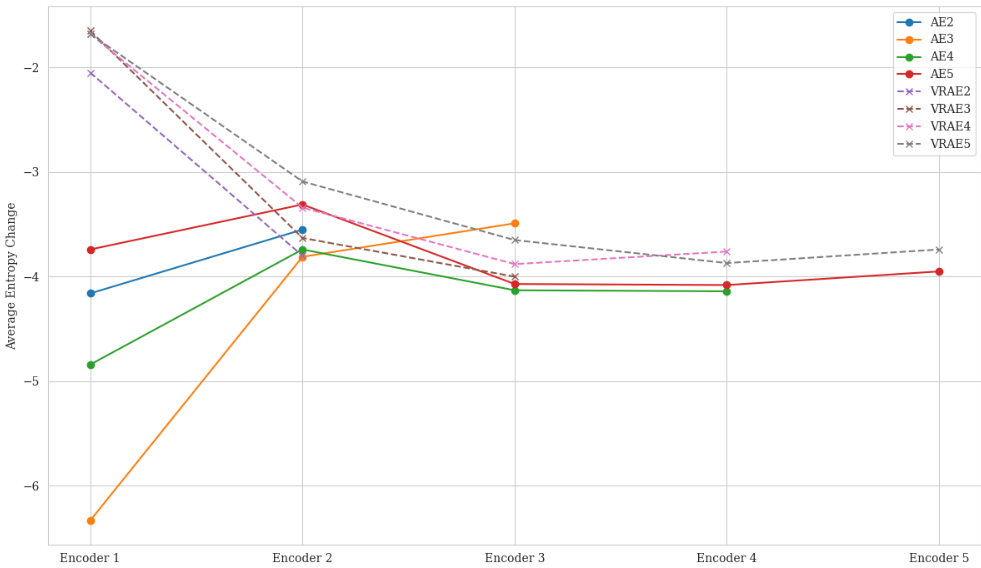
\includegraphics[width=\linewidth]{images/entropy_change.png}
                \caption{Thay đổi Entropy qua các lớp mã hóa}
            \end{figure}
        \end{column}
        \begin{column}{0.5\textwidth}
            \textbf{Quan sát:}
            \begin{itemize}
                \item \textbf{Giai đoạn đầu:} VRAE bắt đầu với mức entropy cao hơn AE
                \item Bảo toàn được nhiều đặc trưng thô và chi tiết vi mô ngay từ đầu
                \item \textbf{Sự ổn định:} Giảm entropy mượt mà, nhất quán
                \item Tránh "sụp đổ thông tin" (information collapse) quá sớm
            \end{itemize}
            
            \textbf{Ví dụ VRAE3:}
            \begin{itemize}
                \item Giảm dần: -1.5 $\rightarrow$ -3.7
                \item Trái ngược AE3: -6.3 $\rightarrow$ -3.5 (giảm đột ngột)
            \end{itemize}
        \end{column}
    \end{columns}
\end{frame}

% \begin{frame}{Phân tích Trade-off (Pareto Front)}
%     \begin{columns}
%         \begin{column}{0.5\textwidth}
%             \begin{figure}
%                 \centering
%                 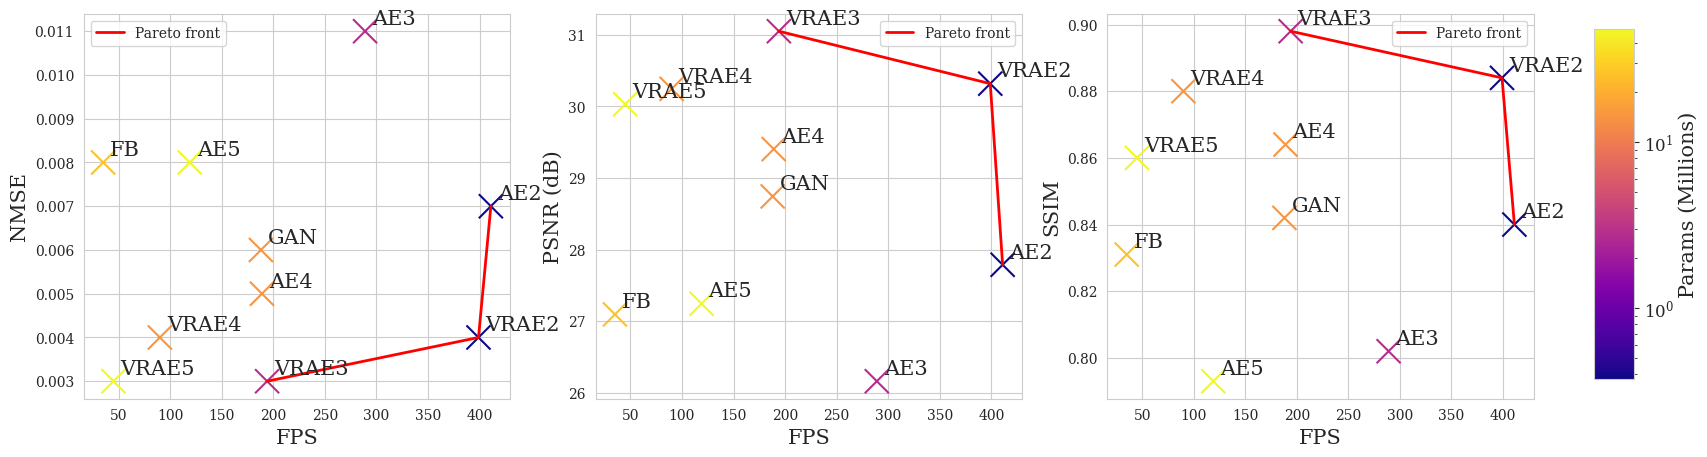
\includegraphics[width=\linewidth]{images/pareto.png}
%                 \caption{Pareto Front: Chất lượng vs Tốc độ}
%             \end{figure}
%         \end{column}
%         \begin{column}{0.5\textwidth}
%             \textbf{Đánh đổi giữa:}
%             \begin{itemize}
%                 \item Hiệu suất tái tạo (PSNR/SSIM)
%                 \item Tốc độ suy luận (FPS)
%             \end{itemize}
            
%             \vspace{0.3cm}
%             \textbf{Kết quả:}
%             \begin{itemize}
%                 \item VRAE2 và VRAE3 nằm trên \textbf{đường biên tối ưu}
%                 \item Kết hợp tốt nhất giữa độ chính xác và hiệu năng
%                 \item GAN và FB: Tham số lớn nhưng hiệu quả thấp hơn
%             \end{itemize}
%         \end{column}
%     \end{columns}
% \end{frame}



\section{Hướng phát triển tương lai}

\begin{frame}{Hướng phát triển tương lai}
    \small
    \begin{itemize}

        \item \textbf{Kiến trúc độ sâu thích ứng:}
        \begin{itemize}
            \item Tự động điều chỉnh độ sâu theo độ phức tạp ảnh đầu vào
            \item Tiết kiệm tài nguyên cho ảnh ít nhiễu
        \end{itemize}
        \item \textbf{Khôi phục video thời gian thực:}
        \begin{itemize}
            \item Mở rộng từ ảnh tĩnh sang luồng video
            \item Tận dụng thông tin liên quan giữa các khung hình
        \end{itemize}
        \item \textbf{Đánh giá đa dạng:}
        \begin{itemize}
            \item Thử nghiệm trên nhiều bộ dữ liệu biển số khác nhau
            \item Điều kiện thời tiết khắc nghiệt (mưa lớn, sương mù)
        \end{itemize}
    \end{itemize}
\end{frame}

% \begin{frame}{Hướng phát triển tương lai (2)}
%     \small
%     \begin{itemize}
%         \item \textbf{Khôi phục video thời gian thực:}
%         \begin{itemize}
%             \item Mở rộng từ ảnh tĩnh sang luồng video
%             \item Tận dụng thông tin liên quan giữa các khung hình
%         \end{itemize}
%         \item \textbf{Đánh giá đa dạng:}
%         \begin{itemize}
%             \item Thử nghiệm trên nhiều bộ dữ liệu biển số khác nhau
%             \item Điều kiện thời tiết khắc nghiệt (mưa lớn, sương mù)
%         \end{itemize}
%     \end{itemize}
% \end{frame}


\section{Kết luận}

\begin{frame}{Kết luận}
    \textbf{Đóng góp chính:}
    \begin{enumerate}
        \item Đề xuất kiến trúc \textbf{VRAE} tích hợp:
        \begin{itemize}
            \item Kết nối dọc (Vertical Residual)
            \item Khối bổ trợ (Auxiliary Block)
            \item Cơ chế hội tụ đặc trưng đa cấp
        \end{itemize}
        \item Giải quyết bài toán cân bằng:
        \begin{itemize}
            \item Độ chính xác phục hồi (PSNR > 31 dB, SSIM > 0.89)
            \item Chi phí tính toán (194 FPS với VRAE3)
        \end{itemize}
        \item Vượt trội so với các phương pháp hiện có:
        \begin{itemize}
            \item Tăng PSNR ~20\% so với AE cùng độ sâu
            \item Vượt GAN và Flow-based về cả chất lượng và tốc độ
        \end{itemize}
        \item Công bố bài báo tại SOICT 2025
    \end{enumerate}
\end{frame}



% \begin{frame}{Công bố khoa học}
%     \begin{block}{Bài báo được chấp nhận}
%         \textbf{Tên bài báo:} "VRAE: Vertical Residual Autoencoder for License Plate Denoising and Deblurring"
        
%         \vspace{0.2cm}
%         \textbf{Hội nghị:} SOICT 2025 (Hội nghị Quốc tế về Công nghệ Thông tin và Truyền thông lần thứ 14)
        
%         \vspace{0.2cm}
%         \textbf{Tác giả:} Nguyễn Tất Cường (tác giả chính)
        
%         \vspace{0.2cm}
%         \textbf{Năm:} 2025
%     \end{block}
    
%     \begin{figure}
%         \centering
%         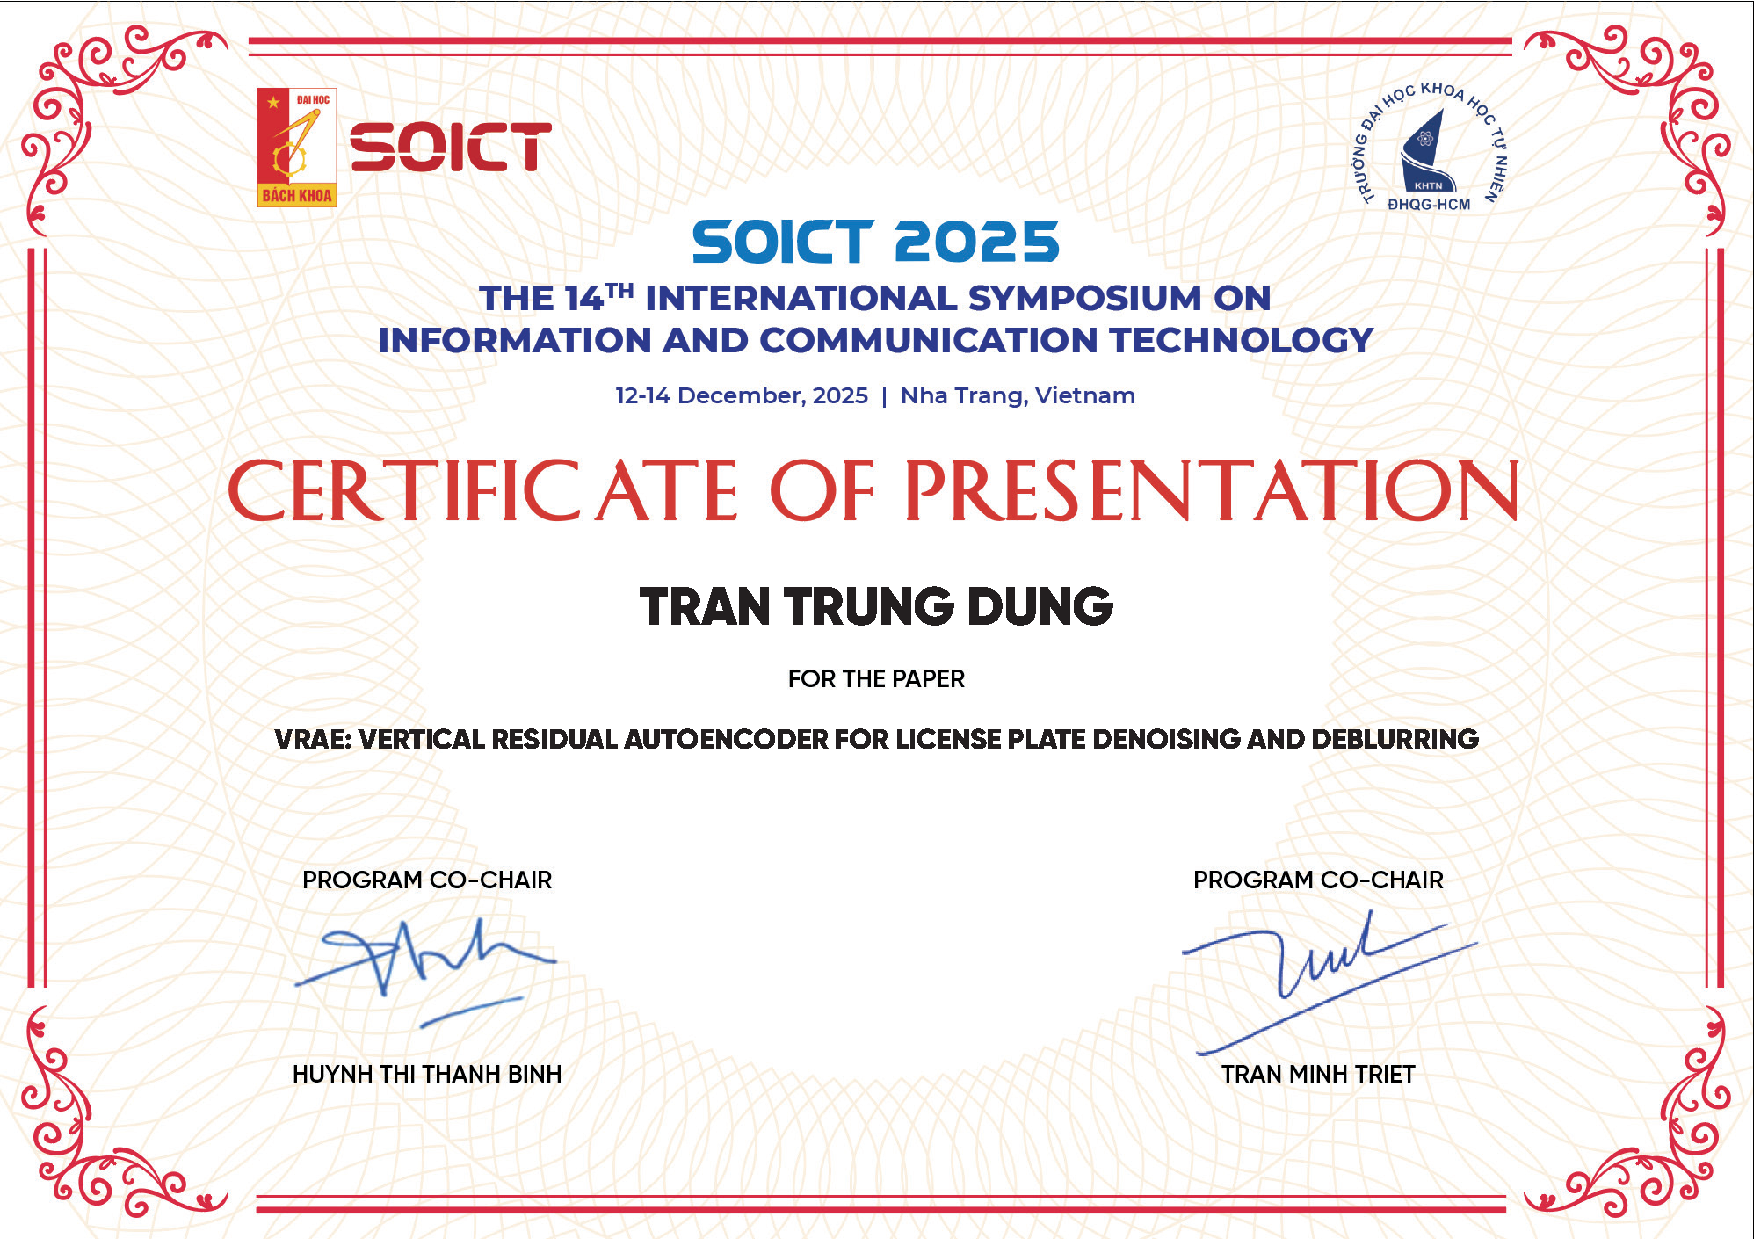
\includegraphics[width=0.5\linewidth]{images/certificate.pdf}
%         \caption{Minh chứng bài báo được trình bày tại SOICT 2025}
%     \end{figure}
% \end{frame}





% \section{Tài liệu tham khảo}
\begin{frame}{Tài liệu tham khảo}
    \nocite{vincent2008, goodfellow2014, kingma2018, shannon1948}
    \bibliographystyle{plain}
    \bibliography{refs.bib}
\end{frame}

\begin{frame}{~}
    \centering
    \Large \color{hustred}{Cảm ơn Thầy Cô và các bạn đã chú ý lắng nghe!}
\end{frame}


\end{document}








